\section{Experiments}

\label{sec:experiments}

\subsection{Test Design}

\subsubsection{Research Questions}

\label{subsubsec:evaluation_questions}

We test the three steps that make a rule useful: acquire it, generate
its candidate, and execute it to repair a record.
\textbf{RQ1:} How does learned scheduling compare with simple policies
under fixed rules and graph operations?
\textbf{RQ2:} Which reward terms and policy parts change repair and
correct facts kept?
\textbf{RQ3:} What do the two prompts add at equal call budgets,
and which repairs do their candidates support?

The fixed rule library tests RQ1 and RQ2. Saved generation responses,
rule execution, and document tests address RQ3. The document stage uses
fixed schedules and measures candidate coverage.

\subsubsection{Data and Test Rules}

\label{subsubsec:testset}

The policy environment uses 450 balanced TNEWS/CLUE documents, 30 per
category. The graph has 873 nodes and 1,083 relations. Independent seeds
add isolated nodes, duplicate edges, invalid relations, and edges with
missing endpoints. The reward study has twenty development scenarios
and thirty test scenarios from the same base graph. The earlier ten
scenarios supply action tests and historical component results.
A separate 180-case set supplies online rule precision and recall.
Acquisition activates stored modules. After detection, relation repair
reads the environment's private restoration record.

The rule study uses 9,456 successful saved responses: deletion and
augmentation for each of 4,728 government-service documents.
RuleTest-94 has 30 clean and 64 defective records with stored expected
labels. DocRED supplies entity types and source text for document tests
(Appendix~\ref{app:docred_pilot}). Appendix~\ref{app:supporting_checks}
gives further structural and extraction tests.

\subsubsection{Replay Records}

\label{subsubsec:runtime_reproducibility}

Before training, we fix sources, seeds, costs, and episode budgets.
A second manifest records model and scorer hashes before the test run.
We retain all predefined policies and failed outcomes. Policies receive
current observations and masks. The scorer uses reference labels.
Appendix~\ref{app:reward_protocol} gives splits and inference rules.
Appendix~\ref{app:artifact_index} lists saved steps and replay commands.
Local training and saved-output replay use zero API requests.
Generation costs have separate records.

\subsection{Learning Graph and Rule Actions}

\label{subsec:rl_results}

\subsubsection{Checking the Reward}

The earlier count-penalty Double DQN introduces zero violations.
Its ten saved action logs also contain zero relation repairs and leave
61.3 invalid relations per graph. We try each allowed action from saved
states. Twenty Double-DQN and heuristic action logs give 2,214 one-step
trials, including 311 relation-repair trials. These trials run after
the policy evaluation.

All 155 allowed relation-repair trials from Double-DQN states have
negative immediate reward with the count penalty. Across these overlapping
trials, repairs create 443 duplicate edges. They add zero wrong reference
facts and remove zero correct facts. Mean immediate reward changes from
$-0.01990$ with the count penalty to $+0.00821$ with the rate penalty.
Repair followed by duplicate removal gives two-step discounted returns
of $-0.01781$ and $+0.01030$. The count penalty blocks useful repair
by charging for temporary duplicates.

\begin{figure*}[t]
\centering
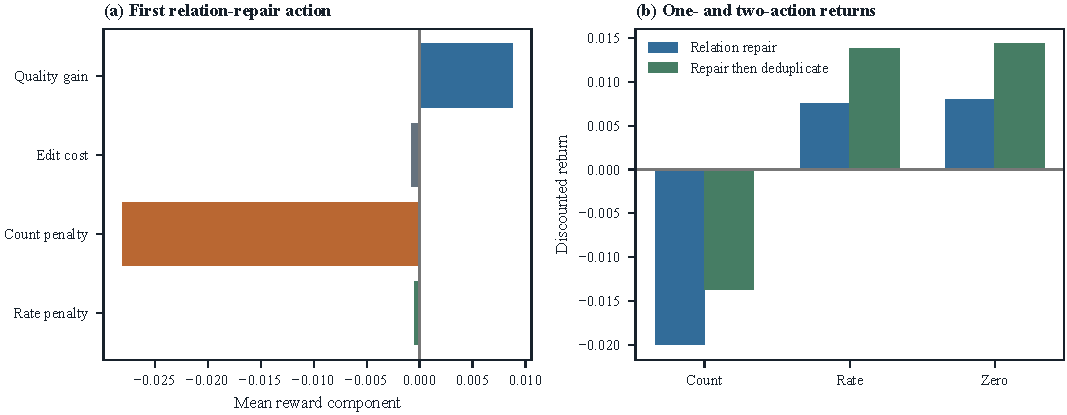
\includegraphics[width=0.98\textwidth]{figure/experiments/reward_action_audit.pdf}
\caption{Reward parts on ten earlier scenarios. Each trial starts from the corrupted input with four high-precision rules active. (a) Mean quality gain, edit cost, and each penalty for the first relation repair. (b) Return for that action and for repair followed by duplicate removal, with discount 0.95. Panel (a) shows the two penalties separately.}
\label{fig:reward_action_audit}
\end{figure*}

\subsubsection{Policies and Scores}

We train Double DQN with each of the three penalties and DQN with
the rate penalty. All eight policies use the same fourteen features,
action mask, and eighteen-step limit.
The \emph{acquire-then-deficit} heuristic gets missing high-precision
modules in mixed, deletion, then augmentation order. It then chooses
the allowed graph action with the largest weighted quality deficit.
Random-valid and rule-first-valid give two further schedules.

The one-step ridge baseline fits quality gain, edit count, and new-error
rate burden for each action. Each of ten fits uses 250 episodes of
uniform allowed-action exploration. Neural models have the same episode
budget. Ridge receives the fourteen public features and observed reward
parts. Each action has its own training-data standardization.
The ridge coefficient is one, with an unpenalized intercept.
At inference, predicted edits and burden are clipped at zero.
The policy chooses the highest predicted rate reward, including call cost.
Ridge uses separate random action logs. Policy inputs contain current
features and masks.

Let $F^*$, $F_0$ and $F_T$ be unique triple sets for the clean reference,
corrupted input, and final graph. The primary reference score is

\begin{equation}
\mathrm{F1}_{\mathrm{triple}}=\frac{2|F_T\cap F^*|}{|F_T|+|F^*|}.
\end{equation}

The second primary score counts original invalid edge IDs that remain
with their reference relation restored. Removed edges receive zero
restoration credit, including repaired copies removed during deduplication.
Triple F1 counts unique facts. The share of correct facts kept is
$|F_T\cap F_0\cap F^*|/|F_0\cap F^*|$. The clean extraction and controlled
corruptions supply these reference sets.

We also count remaining errors, new errors by family, correct and wrong
fact changes, edits, and acquisition units. Final joint quality and
quality over the shared budget are

\begin{equation}
\begin{aligned}
\bar Q_t&=\frac{Q(G_t)+0.4Q_{\mathrm{online}}(R_t)}{1.4},\\
\mathrm{AUC}_{18}&=\frac1{18}\sum_{t=0}^{17}\frac{\bar Q_t+\bar Q_{t+1}}2.
\end{aligned}
\end{equation}

For an early stop, the final quality is carried forward to step eighteen.
All evaluated returns use the rate penalty. The archive also stores returns
under count and zero penalties. Acquisition units measure simulated cost.
Actual API requests are zero.

% Begin merged tables/reward_validation.tex
\begin{table*}[t]
\centering
\caption{Rewards on thirty new corruptions of the same base graph. Means and standard deviations use ten run-seed means. F1 checks unique reference triples. Restoration counts original bad edges kept with their reference relation. All returns use the rate penalty.}
\label{tab:reward_validation}
\footnotesize
\setlength{\tabcolsep}{3pt}
\begin{tabular*}{\textwidth}{@{\extracolsep{\fill}}lrrrrrr@{}}
\toprule
Policy & Triple F1 (\%) & Restored (\%) & Facts kept (\%) & New errors & Calls & Return \\
\midrule
DDQN (count) & $94.67\pm0.00$ & $0.00\pm0.00$ & 100.00 & 0.00 & 6.27 & 0.3692 \\
DDQN (rate) & $99.49\pm0.64$ & $94.00\pm12.44$ & 100.00 & 4.20 & 4.42 & 0.3806 \\
DDQN (zero) & $99.75\pm0.31$ & $99.06\pm1.37$ & 100.00 & 4.42 & 4.06 & 0.3803 \\
DQN (rate) & $99.77\pm0.34$ & $96.94\pm6.28$ & 100.00 & 4.33 & 4.21 & 0.3818 \\
One-step ridge & $99.88\pm0.01$ & $97.90\pm0.15$ & 100.00 & 4.37 & 4.04 & 0.3874 \\
Acquire + deficit & $99.91\pm0.00$ & $98.77\pm0.00$ & 100.00 & 4.37 & 4.00 & 0.3877 \\
Rule-first valid & $99.40\pm0.00$ & $94.73\pm0.00$ & 100.00 & 4.27 & 8.00 & 0.3514 \\
Random valid & $97.84\pm0.19$ & $70.72\pm3.03$ & 100.00 & 3.12 & 9.72 & 0.3394 \\
\bottomrule
\end{tabular*}
\end{table*}
% End merged tables/reward_validation.tex


% Begin merged tables/reward_validation_tests.tex
\begin{table*}[t]
\centering
\caption{Rate DDQN minus each baseline in F1 points. Intervals resample ten run-seed means from the same thirty scenarios. Exact sign tests use Holm correction across eight comparisons.}
\label{tab:reward_validation_tests}
\footnotesize
\setlength{\tabcolsep}{3pt}
\begin{tabular*}{\textwidth}{@{\extracolsep{\fill}}llrrr@{}}
\toprule
Baseline & Metric & Difference & 95\% interval & Holm $p$ \\
\midrule
DDQN (count) & Triple F1 & +4.824 & $[+4.403,+5.141]$ & 0.0156 \\
DDQN (count) & Restoration & +94.000 & $[+85.976,+99.919]$ & 0.0156 \\
DDQN (zero) & Triple F1 & -0.255 & $[-0.673,+0.094]$ & 0.9375 \\
DDQN (zero) & Restoration & -5.057 & $[-12.825,+0.509]$ & 0.9375 \\
One-step ridge & Triple F1 & -0.387 & $[-0.810,-0.069]$ & 0.1875 \\
One-step ridge & Restoration & -3.898 & $[-11.927,+2.006]$ & 0.9375 \\
Acquire + deficit & Triple F1 & -0.415 & $[-0.837,-0.099]$ & 0.1875 \\
Acquire + deficit & Restoration & -4.772 & $[-12.796,+1.147]$ & 0.9375 \\
\bottomrule
\end{tabular*}
\end{table*}
% End merged tables/reward_validation_tests.tex


\subsubsection{Policy Results}

Count-penalty Double DQN makes zero relation repairs and leaves 60.03
invalid relations per graph (Table~\ref{tab:reward_validation}).
Its triple F1 is 94.67\%. Rate-penalty Double DQN restores 94.00\% of
original invalid edge copies and reaches 99.49\% F1.
The F1 gain is 4.824 points (95\% CI: $[4.403,5.141]$).
Both primary count--rate tests pass Holm correction ($p=0.0156$).
The rate policy averages 3.92 relation-repair actions and leaves
3.57 invalid relations per graph.

Zero penalty reaches 99.75\% F1 and 99.06\% restoration.
Ridge reaches 99.88\% and 97.90\%. Acquire-then-deficit reaches 99.91\%
and 98.77\%. These three have higher means than rate Double DQN.
The six paired comparisons have Holm-adjusted $p>0.05$
(Table~\ref{tab:reward_validation_tests}). Rate-policy restoration has
a standard deviation of 12.44 points across seed means.
Figure~\ref{fig:reward_validation} shows this variation.

All eight policies keep every initially correct reference fact and add
zero new wrong reference facts. New violations are duplicate edges.
Rate Double DQN adds 4.20 per graph, zero penalty adds 4.42, and
the heuristic adds 4.37. Their discounted returns under the shared rate
reward are 0.3806, 0.3803, and 0.3877. The heuristic uses 4.00 acquisition
units, compared with 4.42 for rate Double DQN.

\begin{figure*}[t]
\centering
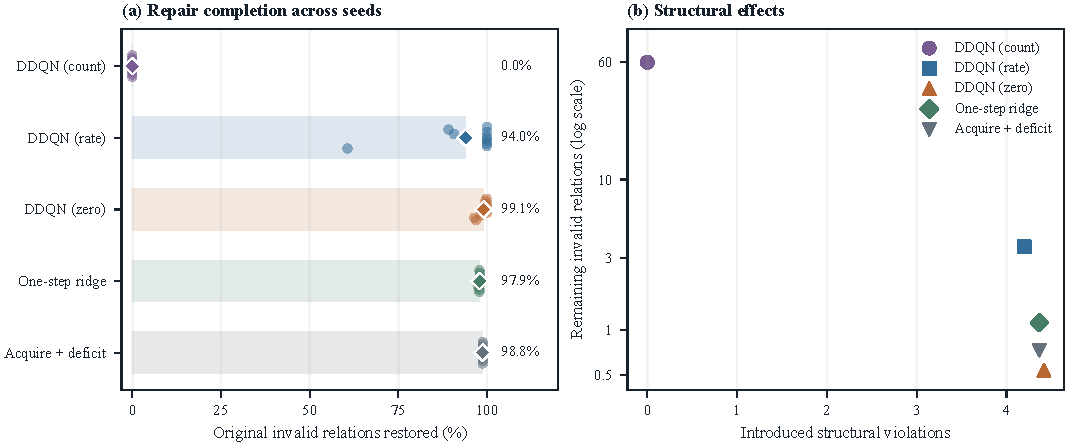
\includegraphics[width=0.98\textwidth]{figure/experiments/reward_validation.pdf}
\caption{Policy behavior on thirty new corruptions. (a) Original invalid edge copies restored and kept. Small dots show ten seed means; diamonds show their average. (b) New structural errors and remaining invalid relations. Each seed mean uses thirty scenarios. Panel (b) averages seeds and uses a log axis.}
\label{fig:reward_validation}
\end{figure*}

\subsubsection{Statistics and Component Tests}

We average the thirty scenarios within each training or run seed.
The statistical units are ten paired seed means. We use 10,000 paired
bootstrap draws and exact two-sided sign randomization over all $2^{10}$
assignments. Holm correction covers eight planned comparisons:
rate Double DQN against count, zero, ridge, and acquire-then-deficit
for both primary scores. Each interval measures seed variation on
the fixed test set. Fixed schedules repeat the same outcome across seeds.

Appendix~\ref{app:impl} gives the earlier count-penalty component tests.
The next tests use the rate reward to measure features, masking,
acquisition cost, and penalty size.

% Begin merged sections/rate_ablation.tex
\subsubsection{Component Tests with the Rate Reward}

\label{sec:rate_ablation}

We test five changes: remove graph features, remove rule features,
remove the action mask, remove training call cost, or use a small count
penalty. Ten seeds and 250 episodes per setting train fifty new models.
The ten existing rate-DDQN checkpoints give the full-policy baseline.
Thirty further corruptions of the same base graph give 2,100 outcomes,
including the heuristic. We evaluate every fixed model.

Feature removal sets the chosen inputs to zero during training and testing.
Other inputs and the mask stay available. The no-mask setting chooses
from all eight actions during action selection and target updates.
Unavailable graph actions can leave the graph unchanged. Repeated
acquisition can incur call cost. The no-call-cost setting removes that
training reward term. Evaluation uses the shared rate reward.

\begin{table}[t]

\centering

\caption{Rate-reward component tests. Values average ten seed means, each from thirty shared scenarios. Calls count simulated acquisition units. API requests are zero.}

\label{tab:rate_ablation}

\scriptsize

\begin{tabular}{lrrrr}

\toprule

Setting & F1 & Restoration & Calls & Unavailable \\

\midrule

Rate DDQN & 0.9952 & 0.9377 & 4.45 & 0.00 \\

No graph features & 0.9941 & 0.8938 & 4.10 & 0.00 \\

No rule features & 0.9775 & 0.6682 & 7.39 & 0.00 \\

No action mask & 0.9702 & 0.5776 & 6.23 & 8.26 \\

No call penalty & 0.9854 & 0.7686 & 5.54 & 0.00 \\

Small count penalty & 0.9905 & 0.9214 & 4.89 & 0.00 \\

Acquire-then-deficit & 0.9991 & 0.9884 & 4.00 & 0.00 \\

\bottomrule

\end{tabular}

\end{table}

Removing the mask lowers F1 by 2.50 points
(95\% seed-bootstrap CI: $[-3.45,-1.62]$; Holm $p=0.0234$).
It gives 8.26 unavailable choices per episode. This is the one comparison
with adjusted $p<0.05$ among twelve F1 and restoration tests.
Removing rule features lowers mean F1 and raises acquisition cost;
its adjusted $p>0.05$. Every setting keeps all initially correct
reference facts. The heuristic reaches the highest mean F1, 99.91\%.

\paragraph{Testing penalty size.}

Twenty development rollouts sample allowed actions uniformly.
We set the count coefficient to total rate burden divided by total new
violations: $\alpha=0.000164493$. Calibration uses observed graph changes.
Small-count DDQN reaches 99.05\% F1; rate DDQN reaches 99.52\%.
The paired difference is $-0.47$ points
(CI: $[-1.73,0.46]$, Holm $p=1$). The interval includes zero at
the base graph size.

\begin{figure*}[t]

\centering

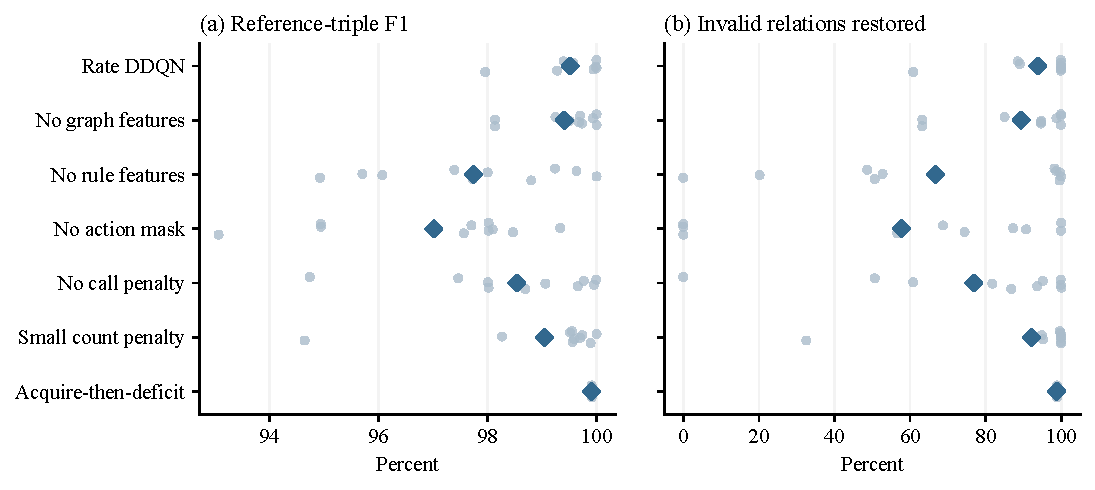
\includegraphics[width=0.93\textwidth]{figure/experiments/rate_ablation.pdf}

\caption{Rate-reward component tests and small-count control. Dots show ten training-seed means; diamonds show their average. Each mean uses thirty shared scenarios. The heuristic uses a fixed rule.}

\label{fig:rate_ablation}

\end{figure*}
% End merged sections/rate_ablation.tex


% Begin merged sections/scale_control.tex
\subsubsection{Fixed Policies on Larger Graphs}

\label{sec:scale_control}

We build one, two, four, and eight disjoint copies of the clean base graph.
Each copy has separate node IDs. The largest input has 6,984 nodes and
8,664 edges. At each size, ten policy seeds and five shared corruption
seeds compare rate, original-count, and small-count DDQN with
acquire-then-deficit. This gives 800 outcomes. All models train at
the base size. The test uses repeated content at larger graph sizes.

\begin{figure*}[t]

\centering

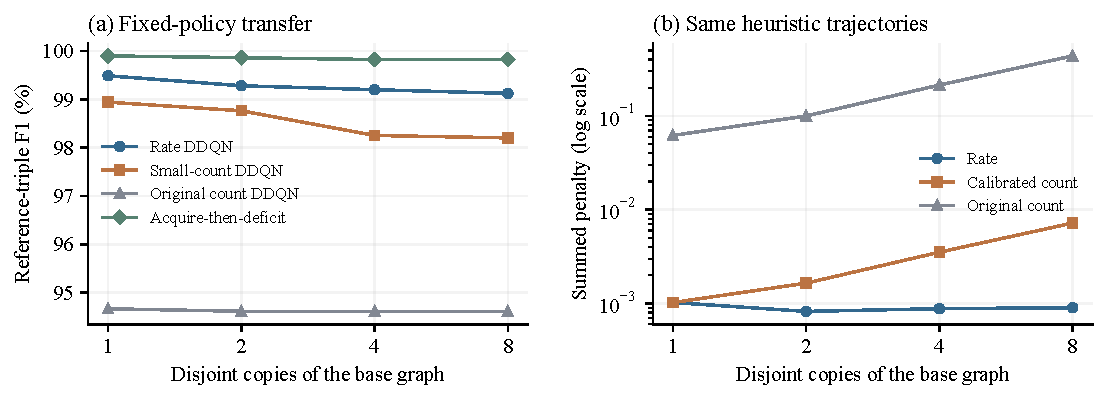
\includegraphics[width=0.94\textwidth]{figure/experiments/scale_control.pdf}

\caption{Graph-size test with disjoint copies. (a) Mean F1 across ten model seeds and five scenarios per size. (b) Three penalties on the same heuristic action logs. All models train at the base size.}

\label{fig:scale_control}

\end{figure*}

\begin{table}[t]

\centering

\caption{Heuristic time and memory, three runs per size. Time includes construction and actions with \texttt{tracemalloc}. Memory counts peak traced Python allocations during these steps. The clean graph and native tensor storage are excluded.}

\label{tab:scale_resources}

\scriptsize

\begin{tabular}{rrrr}

\toprule

Clean edges & Copies & Time (s) & Memory (MiB) \\

\midrule

1,083 & 1 & 0.881 & 1.32 \\

2,166 & 2 & 1.839 & 2.89 \\

4,332 & 4 & 4.126 & 5.46 \\

8,664 & 8 & 8.805 & 11.35 \\

\bottomrule

\end{tabular}

\end{table}

On the same heuristic action logs, the small-count burden grows by
7.06 times from one to eight copies. The rate burden changes by
0.88 times. These scores measure penalty scaling with matched actions.
% End merged sections/scale_control.tex


\subsection{Candidates from Two Prompts}

\label{subsubsec:dual_strategy_ablation}

\subsubsection{Shared Documents and Equal Calls}

The paired archive has 32,955 distinct deletion candidates and 41,683
augmentation candidates. Their union has 71,656. These totals include
entity and relation declarations. The union is 71.9\% larger than
augmentation alone. It uses 9,456 calls, compared with 4,728.

Equal-call tests use budgets of 100, 500, 1,000, 2,000, and 4,000.
We use thirty seeded shuffles of the paired document list.
One strategy processes $B$ documents once each. Dual generation processes
the first $B/2$ documents with both prompts. The call count is equal;
the document count differs. The saved code removes identical candidates
and counts declarations apart from constraints.
Table~\ref{tab:equal_budget} gives selected budgets.
All budgets and sample lists are released.

% Begin merged tables/offline_budget.tex
\begin{table}[t]
\centering
\caption{Equal-call candidate counts, averaged over thirty document shuffles. Declarations give entity and relation types. Constraints give patterns or statements.}
\label{tab:equal_budget}
\footnotesize
\setlength{\tabcolsep}{3pt}
\begin{tabular*}{\columnwidth}{@{\extracolsep{\fill}}rlrrr@{}}
\toprule
Calls & Strategy & Docs & Decl. & Constraints \\
\midrule
100 & Deletion & 100 & 468 & 702 \\
100 & Augmentation & 100 & 501 & 857 \\
100 & Dual & 50 & 512 & 795 \\
1000 & Deletion & 1000 & 2634 & 6044 \\
1000 & Augmentation & 1000 & 2887 & 7787 \\
1000 & Dual & 500 & 2970 & 7126 \\
4000 & Deletion & 4000 & 7249 & 21299 \\
4000 & Augmentation & 4000 & 7627 & 28407 \\
4000 & Dual & 2000 & 8081 & 25901 \\
\bottomrule
\end{tabular*}
\end{table}
% End merged tables/offline_budget.tex


Augmentation yields more distinct constraints at every equal-call budget.
At 1,000 calls, its mean is 7,787, compared with 7,126 for dual generation.
The two prompts add different candidates on the same documents.
The next stage tests which candidates lead to repairs.

\begin{figure*}[t]
\centering
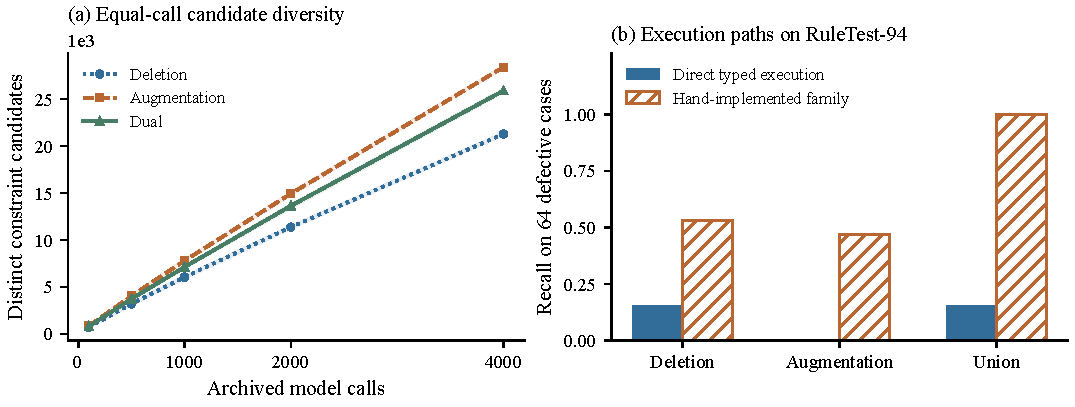
\includegraphics[width=0.98\textwidth]{figure/experiments/offline_rules.pdf}
\caption{Rule-generation scores. (a) Distinct constraints at equal call budgets. Shading shows the 2.5--97.5 percentiles across thirty document shuffles. (b) Recall for direct candidate execution and hand-written family checks.}
\label{fig:rule_quantity}
\end{figure*}

\subsection{Executing Generated Rules}

\label{subsec:generated_rule_transfer}

We test candidate execution, repairs from each strategy, and the effect
of acquisition order.

\subsubsection{Direct Execution of Saved Patterns}

\label{sec:rule_execution_audit}

The archive contains 181,851 candidate copies. Exact allowed and forbidden
type patterns compile to 18,143 distinct rules. Each retains its document,
strategy, response line, category, and position. Two distinct patterns
match RuleTest-94. Of 32,360 compilable copies, 32,348 use terms absent
from the relevant test positions. Nine use test vocabulary but match
zero records; three match a record. The archive and suite thus share
few applicable patterns.

% Begin merged tables/offline_execution.tex
\begin{table}[t]
\centering
\caption{Direct execution of saved type patterns on RuleTest-94: 64 defective and 30 clean cases.}
\label{tab:direct_execution}
\footnotesize
\setlength{\tabcolsep}{3pt}
\begin{tabular*}{\columnwidth}{@{\extracolsep{\fill}}lrrrrr@{}}
\toprule
Strategy & Patterns & TP & FP & Recall & F1 \\
\midrule
Deletion & 5794 & 10 & 0 & 0.156 & 0.270 \\
Augmentation & 12617 & 0 & 0 & 0.000 & 0.000 \\
Dual & 18143 & 10 & 0 & 0.156 & 0.270 \\
\bottomrule
\end{tabular*}
\end{table}
% End merged tables/offline_execution.tex


The union detects 10 of 64 defects and flags zero of 30 clean cases.
Recall is 0.156 and F1 is 0.270. Augmentation makes zero positive
predictions; its precision is undefined. Allowed patterns grant allowed rules.
A conflicting allowed rule and forbidden rule cause the checker to skip
the decision. This suite has zero conflicts. Logs keep unsupported and
malformed candidates. Each strategy is scored on all 94 cases.

\subsubsection{Generated Rules in a Repair Loop}

% Begin merged tables/math_revision_bridge.tex
\begin{table*}[t]
\centering
\caption{Saved generated rules on RuleTest-94. Removal deletes records flagged by a forbidden type rule.}
\label{tab:rule_bridge}
\footnotesize
\setlength{\tabcolsep}{3pt}
\begin{tabular*}{\textwidth}{@{\extracolsep{\fill}}lrrrr@{}}
\toprule
Packet & Rules & Defect removals & Clean removals & Retained \\
\midrule
Deletion & 5794 & 10 & 0 & 84 \\
Augmentation & 12617 & 0 & 0 & 94 \\
Union & 18143 & 10 & 0 & 84 \\
\bottomrule
\end{tabular*}
\end{table*}
% End merged tables/math_revision_bridge.tex


The interface in Section~\ref{sec:rule_bridge_method} activates exact saved
type patterns on RuleTest-94. It updates detections and the removal mask,
removes allowed targets, and saves the next state. Deletion activates
5,794 patterns, augmentation 12,617, and the union 18,143.
Deletion and the union each remove ten defective records and zero clean
records. Augmentation changes zero records. All thirty clean records
remain. Removed records have no replacements.

Four fixed schedules change acquisition order and repair timing.
All give the same final result. Both matching patterns come from deletion:
one allowed rule matches ten records and one forbidden rule flags another ten.
Augmentation matches zero records.

% Begin merged tables/rule_integration_coverage.tex
\begin{table*}[t]
\centering
\caption{Type-rule coverage on RuleTest-94 and three CSV snapshots. All 18,143 patterns are available. Raw snapshots have zero typed records, so the checker skips them.}
\label{tab:rule_integration_coverage}
\footnotesize
\setlength{\tabcolsep}{3pt}
\begin{tabular*}{\textwidth}{@{\extracolsep{\fill}}lrrrr@{}}
\toprule
Input & Records & Typed & Matching rules & Flagged \\
\midrule
RuleTest-94 & 94 & 94 & 2 & 10 \\
Government & 17,939 & 0 & 0 & 0 \\
Finance & 8,180 & 0 & 0 & 0 \\
Environment & 151 & 0 & 0 & 0 \\
\bottomrule
\end{tabular*}
\end{table*}
% End merged tables/rule_integration_coverage.tex


All 26,270 edge copies in the three raw snapshots lack required endpoint
types. The checker therefore skips them
(Table~\ref{tab:rule_integration_coverage}). Appendix~\ref{app:bridge_coverage}
gives the type-source audit and sixteen schedule traces.
The interface loads saved banks and executes fixed schedules.

\begin{figure*}[t]
\centering
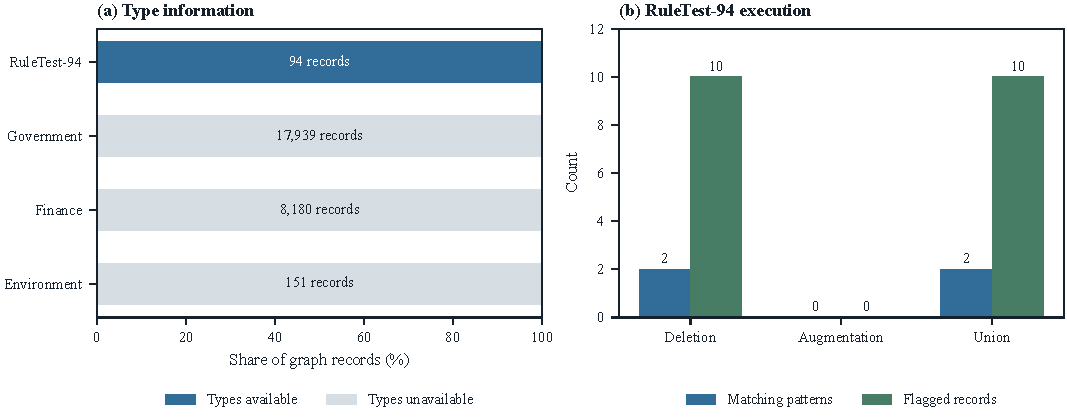
\includegraphics[width=0.98\textwidth]{figure/experiments/rule_integration_coverage.pdf}
\caption{Rule coverage. (a) Endpoint types in each snapshot; bar labels give record counts. (b) Matching patterns and flagged records in RuleTest-94. The checker skips records with missing types.}
\label{fig:rule_integration_coverage}
\end{figure*}

\subsubsection{Document Development Tests}

\label{subsec:source_development}

The document tests use the four-action environment in
Section~\ref{sec:rule_bridge_method}. The first typed DocRED pilot compiles
rules from both prompts and removes zero records. A source-rule version
then uses ten development pairs with twenty documents, given entity types,
and injected records. It checks quotes against the original source.
The reward counts discovered errors apart from edit-created errors.
The expansion rule requires source-triggered repair in at least two
episodes, higher mean F1, and at least 99\% reference facts kept.
Appendix~\ref{app:docred_v2} gives the protocol and both rounds.

Round 1 raises F1 from 94.42\% to 94.59\%. It keeps 98.34\% of reference
facts and loses four. Round 2 uses the same records and reaches 95.69\%.
It loses zero reference facts and removes seven of 31 injected items.
All seven removals use deletion type rules. Zero source-contradiction
rules compile. Both rounds end at the expansion check.

All-path replay measures the best available schedules
(Table~\ref{tab:offline_loop_ceiling}). In round 1, the highest proxy
return gives 91.63\% reference F1, below stop. In round 2, the best
allowed reference-scored schedule reaches 95.69\%, equal to
acquire-then-repair. Order changes discounted return and intermediate
quality, while the final F1 remains the same.

A new fixed protocol uses twenty other development documents and an
explicit JSON format (Appendix~\ref{app:new_rule_feasibility}).
Thirty-nine of forty Gemma outputs pass the format checks.
Six source-contradiction rules compile. Acquiring both banks then repairing
raises F1 from 94.02\% to 96.63\%. It removes 17 of 28 injected items
and loses four reference facts. The mean share of reference facts kept is 98.14\%, compared
with the 99\% threshold. Source contradictions enable three injected-item
removals and two reference losses at their pre-edit states.
Deletion alone gives the same final graphs with two packets.
Both banks use four packets. Augmentation adds zero unique removals.
The best allowed safe schedule reaches 96.75\% F1, 0.12 points above
the strongest fixed schedule. This run also ends at the expansion check.

Admission replay tests the same candidates
(Appendix~\ref{app:rule_admission}). Source-link checks keep all 407 rules
and reproduce the repairs. The independent-approval registry is empty,
and the hard-schema mapping is absent. Both approval settings keep
zero rules. F1 stays at 94.02\%, with zero losses and zero repairs.

\subsection{Time and Cost}

\label{subsec:runtime_cost}

Scheduling uses local graph operations and simulated acquisition units.
Its actual API request count is zero. Candidate-count tests use successful
saved responses. Appendix~\ref{app:prompts} lists their recorded metadata.

The two source-development rounds use 80 Gemma requests for 80 responses.
The new follow-up uses forty requests with zero transport failures or
retries. It uses 255,391 prompt tokens and 58,346 completion tokens.
Mean request time is 13.80 seconds, excluding spacing between requests.
Saved-output replay makes zero requests. Packet counts measure replay
acquisition. Appendix~\ref{app:runtime_details} gives training and
extraction times.

\subsection{Discussion}

Reward design changes which repairs the policy completes. The rate
penalty improves over the original count penalty. The action mask raises
final F1. The simple heuristic has the highest mean reference F1.
The small-count control shows the role of penalty size.

Useful acquisition needs rules that match records and allow correct
repairs. The saved archive has few patterns applicable to RuleTest-94.
Raw snapshots also need entity types. With given types, generated rules
repair development inputs. In round 2, the best schedule and
acquire-then-repair have equal final F1. In the new document pairs,
source rules remove injected items and some reference facts.
Augmentation adds zero unique removals. These results point to rule
review and broader useful coverage as the next steps.

The scheduling score uses controlled errors and trusted restoration
records. Document tests score recovery after injected changes.
Independent review can assess rule and edit meaning. New domains can
test transfer. Appendix~\ref{app:supporting_checks} gives structural
and extraction scores.
